
\subsection{A subset-oriented approach}

\begin{frame}[fragile]
\frametitle{A subset-oriented approach}

Our simple pick-a-point approach sometimes led to goals whose hypotheses were
difficult to use effectively

\begin{verbatim}
  (IMPLIES (AND (NORMP C)
                (NORMP HYP)
                (Q-ITE C HYP NIL)
                (NOT (EQUAL (Q-ITE C HYP NIL) HYP))
                HYP
                (NOT (EQUAL C T))
                (NOT (Q-ITE C NIL HYP))
                (NOT (EVAL-BDD C ARBITRARY-VALUES)))
           (NOT (EVAL-BDD HYP ARBITRARY-VALUES))))
\end{verbatim}
\end{frame}


\begin{frame}[fragile]
\frametitle{A graphical view}

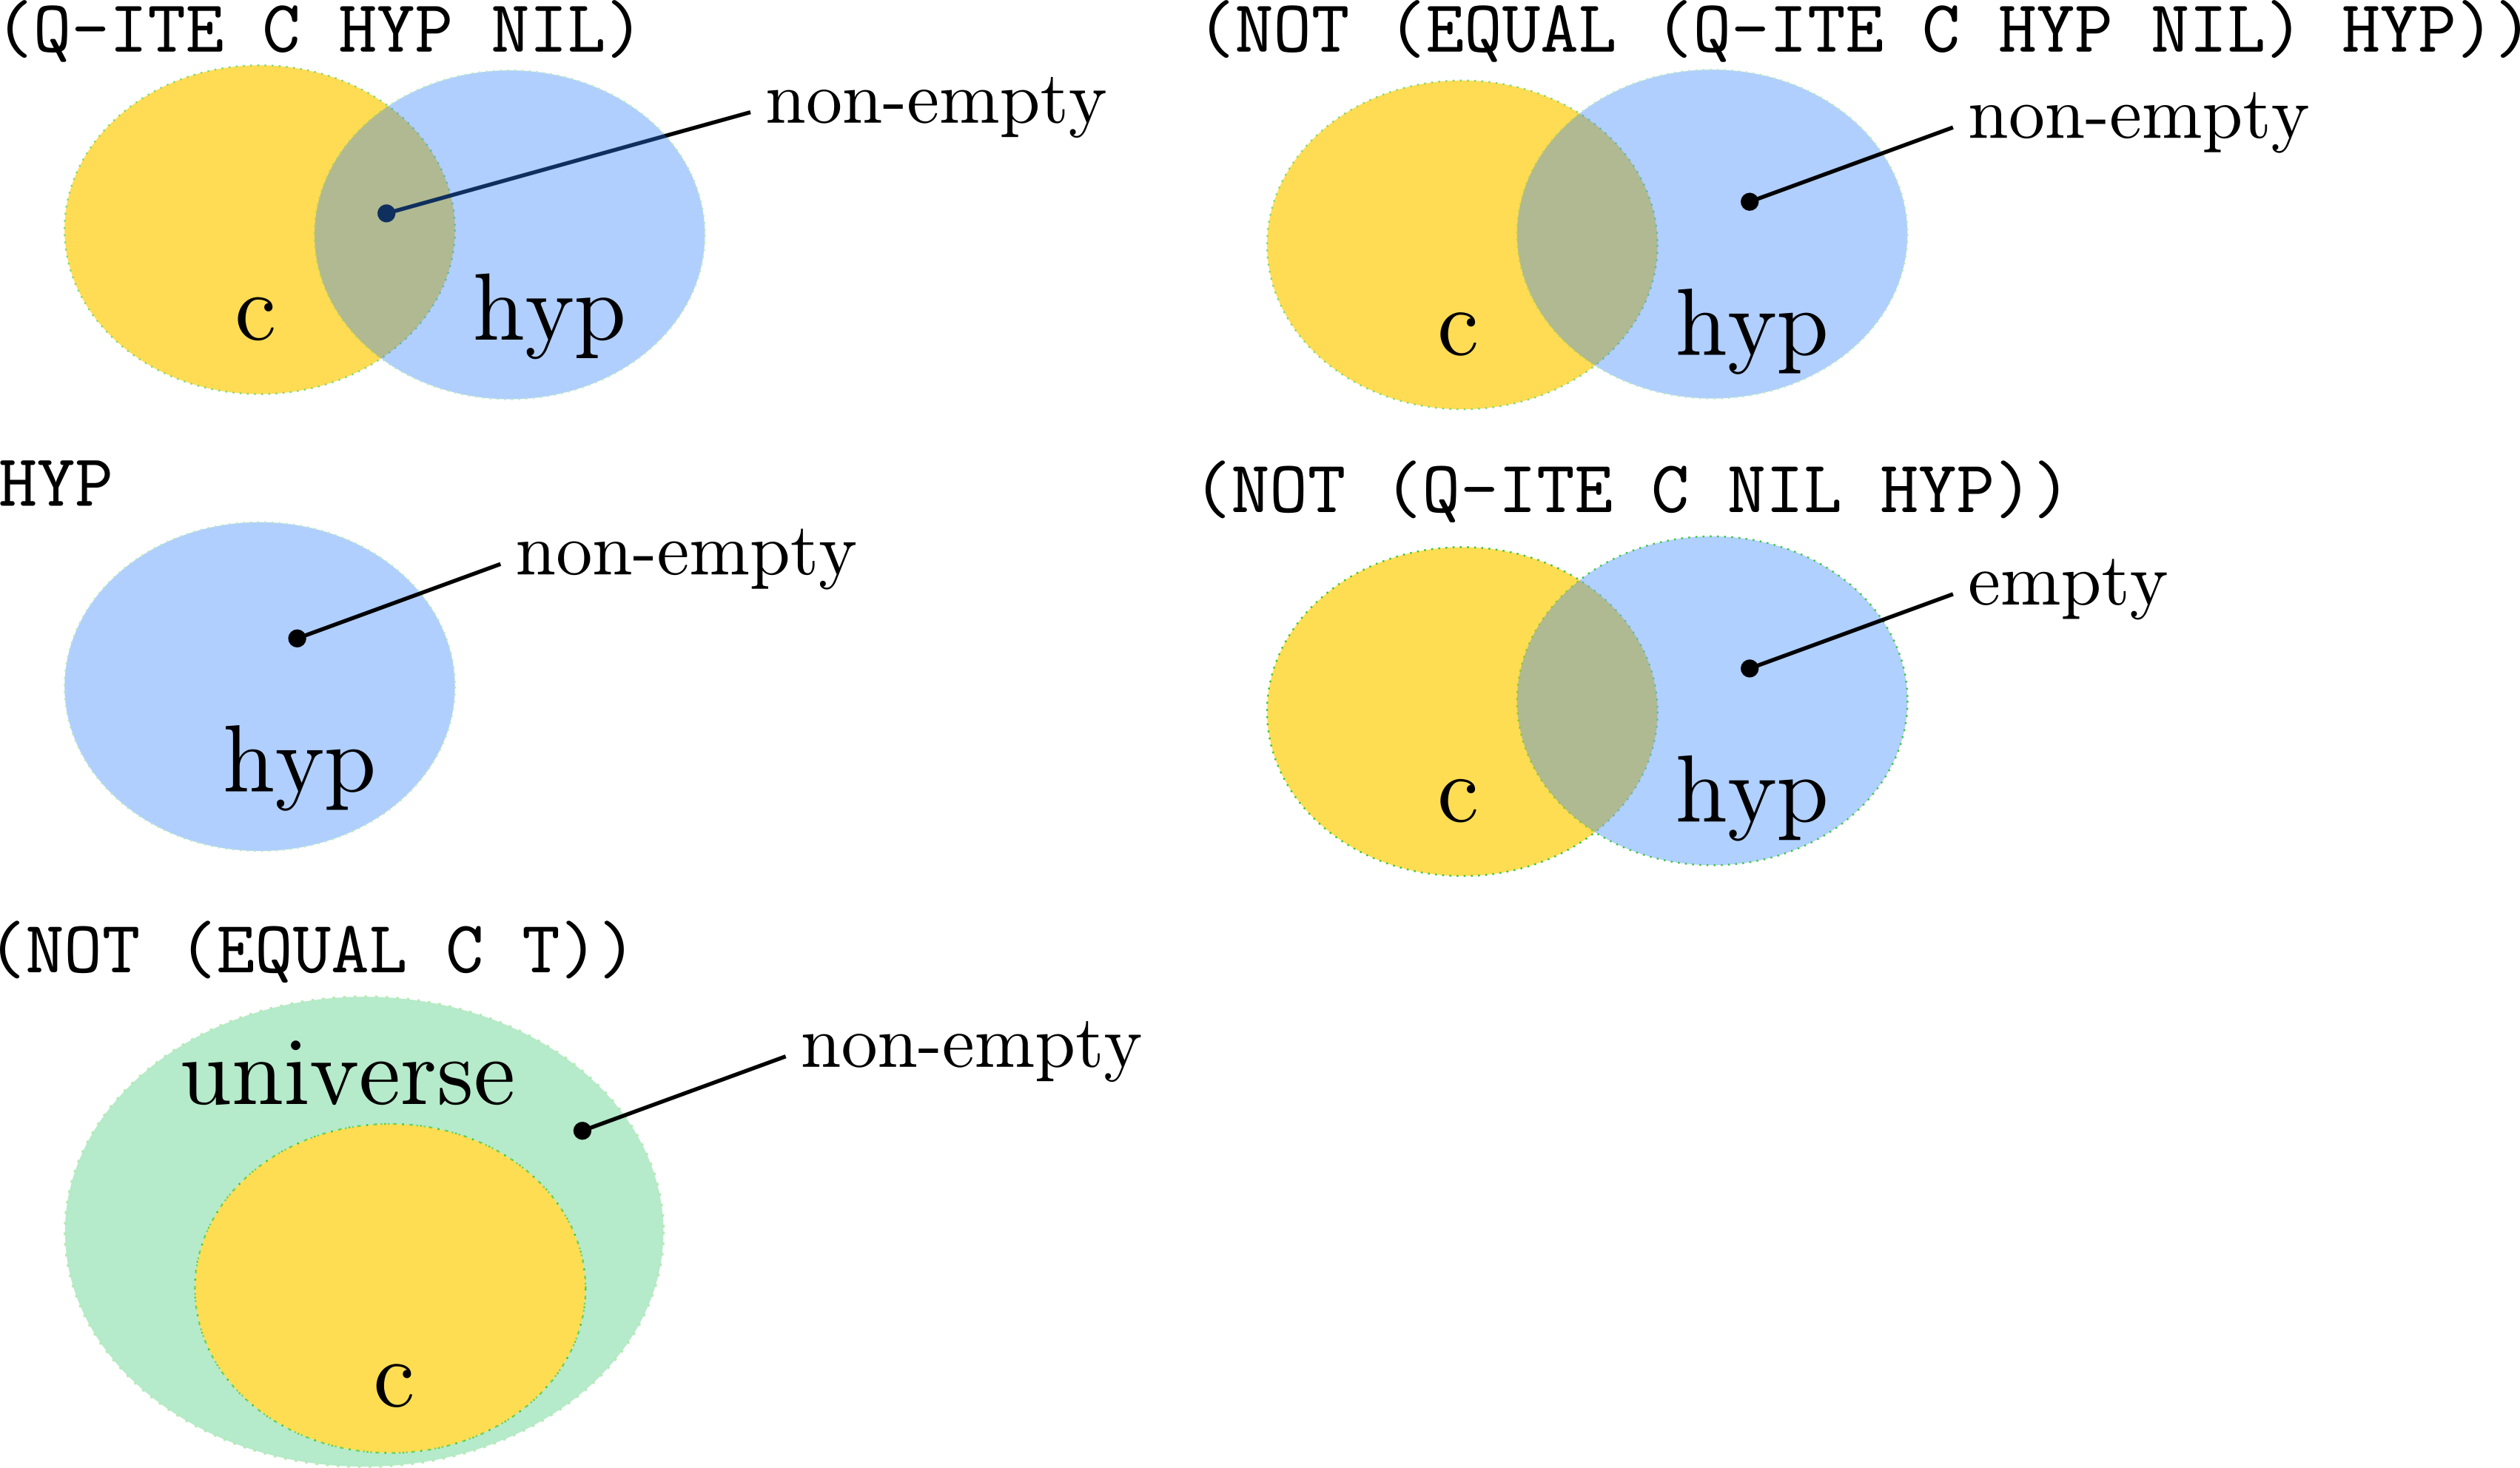
\includegraphics[width=12cm]{venn-diagrams}

\end{frame}



\begin{frame}[fragile]
\frametitle{Subset mode}

\Code{(qs-subset x y)}: $\forall$ \Code{vals} $:$ \Code{(eval-bdd x vals)} $\rightarrow$ \Code{(eval-bdd y vals)}

\begin{itemize}
\item Good properties: reflexive, transitive, membership-preserving
\item Similar pick-a-point approach for proving qs-subset
\end{itemize}

\SmallSkip
\Code{(QS-SUBSET-MODE T)} -- an alternate normal form
\begin{itemize}
\item \Code{(equal x y)} $\Rightarrow$ \Code{(qs-subset x y)} $\wedge$ \Code{(qs-subset y x)}
\item \Code{(not x)} $\Rightarrow$ \Code{(qs-subset x nil)}
\item \Code{x} $\Rightarrow$ \Code{(not (qs-subset x nil))} \\
\quad
\item \Code{(qs-subset (q-and x y) x)}
\item \Code{(qs-subset (q-and x y) y)}
\item \Code{(qs-subset x (q-or x y))}
\item \Code{(qs-subset y (q-or x y))}
\end{itemize}
\end{frame}



\begin{frame}[fragile]
\frametitle{Rewrite rules for subset mode (without {\tt normp} hyps)}
\begin{verbatim}
(equal (qs-subset w (q-ite x y z))
       (and (qs-subset (q-ite w x nil) y)
            (qs-subset (q-ite x nil w) z)))

(implies (and (syntaxp (not (equal y ''nil)))
              (syntaxp (not (equal z ''nil))))
         (equal (qs-subset (q-ite x y z) w)
                (and (qs-subset (q-ite x y nil) w)
                     (qs-subset (q-ite x nil z) w))))

(equal (qs-subset (q-ite x nil y) x)
       (qs-subset y x))

(equal (qs-subset (q-ite x nil y) nil)
       (qs-subset y x))
\end{verbatim}
\end{frame}


\begin{frame}[fragile]
\frametitle{Subset mode in action}

\Code{(not (equal (q-ite c hyp nil) hyp))} $\rightarrow$ \Code{(not (qs-subset hyp c))}
{\footnotesize \begin{verbatim}
  (not (equal (q-ite c hyp nil) hyp))
  ==> (not (and 1. (qs-subset (q-ite c hyp nil) hyp)
                   ==> t
                2. (qs-subset hyp (q-ite c hyp nil))))
                   ==> (and 2a. (qs-subset (q-ite hyp c nil) hyp)
                                ==> t
                            2b. (qs-subset (q-ite c nil hyp) nil)))
                                ==> (qs-subset hyp c)
  ==> (not (qs-subset hyp c))
\end{verbatim}}


\SmallSkip
\Code{(not (q-ite c nil hyp))} $\rightarrow$ \Code{(qs-subset hyp c)}
{\footnotesize \begin{verbatim}
  (not (q-ite c nil hyp))
  ==> (qs-subset (q-ite c nil hyp) nil)
  ==> (qs-subset hyp c)
\end{verbatim}}

\end{frame}


